\documentclass[11pt]{article}

% ── Page layout ──────────────────────────────────────────────────────────────
\usepackage[a4paper, margin=1in]{geometry}

% ── Fonts and encoding ───────────────────────────────────────────────────────
\usepackage[T1]{fontenc}
\usepackage[utf8]{inputenc}
\usepackage{lmodern}
\usepackage{microtype}

% ── Mathematics ──────────────────────────────────────────────────────────────
\usepackage{amsmath}
\usepackage{amssymb}

% ── Tables ───────────────────────────────────────────────────────────────────
\usepackage{booktabs}
\usepackage{array}
\usepackage{longtable}

% ── Graphics and figures ─────────────────────────────────────────────────────
\usepackage{graphicx}
\usepackage{float}
\usepackage{tikz}
\usetikzlibrary{shapes.geometric, arrows.meta, positioning}

% ── Hyperlinks ───────────────────────────────────────────────────────────────
\usepackage[numbers]{natbib}
\usepackage{hyperref}
\usepackage{textcomp}

\graphicspath{{paper_figures/}}

\title{wildfire\_prediction}
\author{}
\date{}

\begin{document}
\sloppy

\maketitle

\section*{Abstract}

A common problem with machine learning for wildfire prediction is that naively trained models tend to memorize seasonal weather patterns rather than learning the actual environmental conditions that cause fires. To solve this, we introduce \textbf{date-conditional negative sampling}. This approach pairs every actual fire event with non-fire examples drawn from the exact same calendar date. By doing this, we force the model to differentiate between fire and non-fire locations that share the exact same broad weather context. Our controlled experiments demonstrate that this method prevents the model from relying on seasonal shortcuts, resulting in much more stable predictive performance year-round.

To apply this practically, we built a \textbf{day-ahead wildfire risk prediction} system specifically for India. We needed comprehensive historical context, so we aggregated eight years of satellite data from 2018 to 31 October 2025 across several distinct sources. For our ground truth on fire events, we use NASA FIRMS (VIIRS S-NPP, Collection 2). We then provide the weather context using ERA5 reanalysis from the \textit{preceding day} ($D{-}1$) to predict fire risk on day~$D$, ensuring the system forecasts the following day's fire activity rather than diagnosing ongoing conditions. Vegetation health is captured from MODIS, and structural land features from SRTM and ESA WorldCover. Altogether, this pipeline generated approximately 6.9 million labeled training examples across both space and time.

To find the best approach, we evaluated five base classifiers: Logistic Regression, Random Forest, LightGBM, CatBoost, and XGBoost. We also built Voting and Stacking ensembles on top of them. Because we need the model to work reliably in the future, we evaluate all models using a strict time-based holdout---training on data from 2018 to 2023, and testing on 2024 to October 2025 data that the models never saw during training. Ultimately, we deployed the Stacking Ensemble because it achieved the best precision and the highest AUC across our ensemble configurations. Since standard ensemble models often produce uncalibrated scores, we apply Isotonic Regression post-calibration to the raw probability outputs, fitted on a dedicated held-out slice of the training period (October--December 2023) to prevent data leakage. This step substantially reduces the Expected Calibration Error, meaning the final scores can be trusted as true fire probabilities rather than just relative rankings.

Because raw predictions aren't enough for operational use, we use SHAP to understand exactly why the model makes its decisions. We analyze feature importance at a national level, as well as broken down across six distinct ecological zones in India. Through this analysis, we show how the interaction between Vapor Pressure Deficit (VPD) and EVI creates a clear non-linear fire-risk threshold that neither variable captures alone. We also ran a feature ablation study to quantify the value of each data source. This confirmed that combining the fuel stack (EVI and elevation) with the meteorological data provides the strongest signal. Finally, to make these insights actionable, we wrapped the entire system in a FastAPI inference backend and a React-based geospatial dashboard that visualizes daily risk maps.

\section*{Introduction}

Roughly a quarter of India's land is covered by forests and natural vegetation. These ecosystems are highly valuable, both as large-scale carbon sinks and as critical resources for millions of people's livelihoods. However, these areas are experiencing an increasing number of wildfires. This trend is largely driven by climate change, prolonged droughts, existing agricultural burning practices, and rugged terrain that makes containment extremely difficult once a fire starts. Because temperature and rainfall patterns across India are shifting, fire seasons are becoming longer. Furthermore, changes in the monsoon cycle are creating extended dry periods, causing vegetation to lose moisture and become highly flammable. The core problem is that once a fire actually ignites, it spreads incredibly fast. The resulting damage—including biodiversity loss, degraded soil, carbon emissions, and ruined watersheds—scales much faster than the time it takes for emergency teams to respond. Because fires outpace containment efforts, predicting them \textit{before} they happen is essential.

The primary engineering challenge in wildfire management is not detecting a fire that is already burning; existing satellite systems like NASA FIRMS handle detection reliably. The real difficulty lies in anticipating where fires will start days in advance. To do this, we need to pinpoint specific locations that are most likely to ignite given the current weather forecasts, the dryness of the local vegetation, and the underlying terrain structure. Machine learning is a strong fit for this problem because it can automatically map the complex, non-linear relationships between weather inputs (like temperature, humidity, wind, and vapor pressure deficit), vegetation health (using EVI as an indicator for live-plant moisture), static terrain factors (like elevation and slope), and historical fire occurrences. This approach makes sense physically because fire ignition behaves like a threshold rather than a linear gradient. Once conditions pass a specific critical point, tiny shifts in the weather can drastically change the probability of a fire, and tree-based machine learning models are fundamentally designed to detect exactly these types of non-linear thresholds.

A major hurdle when training models for this task is dealing with extreme class imbalance. Because fires are relatively rare events, on any given day, less than 0.1\% of grid cells actually catch fire. If we sample the training data naively, the model gets overwhelmed by negative examples. To address this, we rely on date-conditional negative sampling. Instead of picking random non-fire locations across the whole dataset, we specifically sample our ``non-fire'' training examples from areas that did not burn on the exact same date—and therefore under the same broad weather conditions—as an actual fire event. This constraint forces the model to look past obvious seasonal indicators and learn the precise, localized differences that actually distinguish a fire-prone cell from a safe one.

In summary, this paper combines several practical engineering approaches to build a reliable prediction system: (1) we use a strict train/test split separated by time, ensuring we only evaluate performance on genuinely unseen future data; (2) we implement the date-conditional negative sampling method to manage class imbalance and prevent seasonal memorization; (3) we engineer features heavily based on established fire science, focusing specifically on the weather, vegetation, and terrain variables known to drive ignition; and (4) we systematically compare five standard classifiers, as well as Voting and Stacking ensembles, to measure exactly how much value non-linear modeling and ensembling provide over a simple baseline.

\textbf{Our main contributions:}

\begin{itemize}
    \item We aggregated a training dataset containing approximately 6.9 million samples across an eight-year span (2018--October 2025). We joined NASA FIRMS fire detections, ERA5 weather data (lagged by one day relative to the fire label), MODIS vegetation indices, and static terrain and land-cover information from SRTM and ESA WorldCover. This ensures that every individual training example contains the complete environmental context from the preceding day needed to determine if a fire will start.
    \item We developed a date-conditional negative sampling method. By explicitly matching non-fire training examples to the exact same calendar dates as real fires, we directly handle class imbalance while forcing the model to learn the genuine physical relationships between fire and weather, rather than memorizing seasonal shortcuts. ERA5 weather features for both fire and non-fire samples are drawn from day~$D{-}1$ relative to the label date~$D$, ensuring a consistent one-day forecasting horizon.
    \item We evaluated five diverse classifiers—Logistic Regression (providing a simple, interpretable baseline), Random Forest, LightGBM, CatBoost, and XGBoost—using our strict time-based data split. We then combined these base predictors into Voting and Stacking ensembles, eventually selecting the best-performing configuration to serve as our production model.
    \item We implemented an explanation layer using SHAP to translate complex model predictions into clear, natural-language insights. This ensures the output is actionable and easily understood by on-the-ground forest management teams, rather than just by data scientists.
    \item We engineered a complete end-to-end system, featuring an interactive map-based dashboard. This interface visualizes daily wildfire risk across India, displaying categorical risk tiers, localized feature importance breakdowns, and estimated fire spread directions derived from wind and terrain data.
\end{itemize}

\noindent The rest of the paper is structured logically to explain this pipeline. Section 2 details our methodology, covering our data sources, feature engineering logic, the negative sampling strategy, model architectures, and the overall system workflow. Section 3 presents our experimental results and key findings. Finally, Section 4 concludes the paper and outlines our planned next steps.

\section{Materials and Methods}

\subsection{Data Description and Integration Strategy}

To build a robust prediction model, we integrated five distinct datasets. We selected each dataset because it provides a specific, scientifically validated signal about what drives wildfires. Table~\ref{tab:data_sources} outlines each source, its coverage, and our physical reasoning for including it.

\begin{longtable}{|p{2.8cm}|p{3.6cm}|p{1.8cm}|p{3.9cm}|}
\caption{Data Sources and Scientific Integration Rationale}
\label{tab:data_sources}\\
\hline
\textbf{Data Source} & \textbf{Variables Provided} & \textbf{Coverage} & \textbf{Rationale} \\
\hline
\endfirsthead
\hline
\textbf{Data Source} & \textbf{Variables Provided} & \textbf{Coverage} & \textbf{Rationale} \\
\hline
\endhead
NASA FIRMS (VIIRS S-NPP, C2) & Active fire detections (confidence and radiative power) & 2018--2025 & Ground truth for fire occurrence and validation \\
\hline
ERA5 Reanalysis & 2m temperature, humidity, wind speed, vapor pressure deficit & 2018--Oct~2025, $0.25 \times 0.25$ grid & Physics-driven weather context; consistent interpolation across topographically complex terrain \\
\hline
MODIS EVI & Enhanced Vegetation Index (monthly composites) & 2018--2025 & Live-fuel moisture proxy; disentangles green vegetation from soil background \\
\hline
SRTM / ESA WorldCover & Elevation (m), terrain slope, land-cover class & Static & Terrain controls fire spread rate, fuel moisture retention, and vegetation composition \\
\hline
Open-Meteo API & 24h / 7-day weather forecasts (temperature, humidity, wind) & Real-time & Operational inference; enables next-day and weekly risk visualization \\
\hline
\end{longtable}

\noindent
\subsubsection{Fire Occurrence Ground Truth}

For the ground truth on exactly where and when fires occurred, we use NASA FIRMS' VIIRS S-NPP Collection 2 active-fire product, covering 2018 to 31 October 2025. This satellite system detects active fires globally roughly every 12 hours. Because we need high-quality labels, we exclusively retain detections with a ``nominal'' or ``high'' confidence score (dropping ``low'' confidence detections). In addition, we apply a strict Fire Radiative Power (FRP) threshold, retaining only detections with $\text{FRP} \ge 1.0$ MW. This threshold serves as a standard operational floor to ensure we only train on significant thermal anomalies.

One inherent limitation of the VIIRS sensor is that it cannot detect fires through sufficiently thick cloud cover. On days where cloud obscures the satellite's view, fire detections are simply absent from the FIRMS record; the system has no mechanism to distinguish a genuinely fire-free day from an unobservable one. As a result, cloud-obscured days with underlying fires may enter our date-conditional negative sampling pool and be mislabeled as confirmed no-fire observations. This is a known, unaddressed selection-bias risk arising from the data source itself, not from our pipeline design. We document this limitation explicitly in Section~4 and identify integration of cloud-fraction metadata (e.g., the MODIS MOD35 cloud product) as a target for future work.

A critical design decision in our system is the retention of agricultural burning (such as stubble burning in the Indo-Gangetic Plains during October--November and April--May). Rather than masking out these zones, we intentionally retain these detections as legitimate positives. The rationale is that our model functions as an all-cause fire risk system; agricultural fires still present significant particulate pollution and pose serious spread risks to adjacent vegetation and infrastructure. By including them, the system learns the conditions under which these anthropogenic fires are most likely to ignite and escalate.

Figure~\ref{fig:seasonal_freq} shows the seasonal pattern of wildfire occurrence across India over the 2018--2025 study period. March and April represent the peak fire months (with 698k and 558k detections, respectively), coinciding with the pre-monsoon dry season when vegetation is heavily dehydrated. As expected, the monsoon season (June--September) drives fire occurrences to near zero due to high humidity and rainfall. A secondary, smaller peak occurs in October--November, caused by post-monsoon drying and agricultural burning in specific regions. This bimodal seasonal behavior is exactly why we use cyclical month encoding and date-conditional negative sampling; we want to prevent the model from learning a trivial seasonal shortcut.

\begin{figure}[H]
    \centering
    \includegraphics[width=\textwidth]{fig_seasonal_fire_frequency.png}
    \caption{Monthly wildfire detection frequency across India (2018--2025, NASA FIRMS VIIRS S-NPP Collection 2). March is the peak fire month with 698k detections, driven by the pre-monsoon dry season. The monsoon period (June--September) nearly eliminates fire activity. A secondary peak occurs in October--November due to agricultural burning and post-monsoon drying. This bimodal seasonality motivates the use of cyclical month encoding and date-conditional negative sampling to prevent the model from exploiting trivial seasonal shortcuts.}
    \label{fig:seasonal_freq}
\end{figure}

\subsubsection{Meteorological Reanalysis}

For our meteorological context, we rely on ERA5, which is ECMWF's global atmospheric reanalysis dataset. For every grid cell and day, we extract 2m air temperature, 2m relative humidity, 10m wind speed, and vapor pressure deficit (VPD). We compute VPD directly as the gap between the saturated and actual vapor pressure.

\medskip
\paragraph{Day-lag construction.}
To implement genuine next-day fire risk forecasting, we apply a \textbf{one-day lag} to all ERA5 feature extraction: for a labeled event on day~$D$ (whether a fire detection or a date-conditional negative sample), we extract ERA5 meteorological features from day~$D{-}1$. This ensures the model sees only weather information that would realistically be available before day~$D$'s fire activity begins, rather than concurrent same-day conditions. In an operational deployment, ERA5 reanalysis for day~$D{-}1$ serves as a stand-in for a day-ahead numerical weather prediction---a direct swap that requires no pipeline changes. The lag is applied symmetrically to both positive (fire) and negative (no-fire) samples, preserving the integrity of the date-conditional negative sampling strategy.

We chose these specific variables because fire science research consistently links them to ignition probability. Temperature affects fuel drying rates, humidity dictates fuel moisture, wind speed accelerates fire spread by increasing oxygen supply, and VPD serves as a comprehensive metric for plant water stress. Because of this, VPD acts as a stronger fire-weather indicator than raw humidity alone.

\subsubsection{Vegetation Health Indices}

To measure the state of the vegetation, we use MODIS's Enhanced Vegetation Index (EVI), retrieved via NASA's AppEEARS API. We intentionally selected EVI over the more common NDVI because EVI is more sensitive to actual live-canopy greenness, automatically corrects for atmospheric distortions, and is less skewed by background soil in sparsely vegetated regions. EVI values range from -1 to +1. Values near or above 0.3 indicate healthy, actively growing vegetation, while values below 0.2 indicate sparse or stressed vegetation. We use monthly EVI composites at 1km resolution spanning 2018--2025. 

One engineering challenge with MODIS composites is that they are recorded on an 8-day rolling cycle, meaning they do not align cleanly with ERA5's daily timestamps or standard calendar months. To resolve this, we implemented a custom time-alignment function using the \texttt{cftime} library, mapping each MODIS timestamp to its closest corresponding ERA5 daily record.

\subsubsection{Static Topographic and Land-Cover Layers}

To account for structural terrain factors, we incorporate elevation data from the SRTM digital elevation model (at 30m resolution), which we averaged to match our 0.1-degree grid. For land classification, we rely on ESA WorldCover (10m resolution, 2021 snapshot). This dataset classifies land into 11 standardized categories, such as forests, grasslands, croplands, built-up areas, and water bodies.

\subsubsection{Data Integration and Preprocessing}

Once all raw data was retrieved and cleaned, we merged the layers into a unified geospatial database, standardizing everything onto a 0.1-degree grid covering the entirety of India. We selected this specific resolution as an optimal engineering trade-off: it is fine enough to capture critical local variations in fire risk, yet coarse enough that processing 9.4 million samples remains computationally feasible without requiring specialized distributed hardware.

For every grid cell on every specific date, our pipeline executes the following steps: (1) queries FIRMS to check if a fire occurred, (2) extracts the interpolated ERA5 weather variables, (3) aligns and aggregates the MODIS EVI data, (4) appends the static elevation and land-cover values, (5) executes quality control validations, and (6) constructs the final feature vector. Ultimately, this integration yields 9.4 million labeled cell-day records spanning eight years.

\subsection{Feature Engineering and Physics-Informed Design}

We organized our feature engineering into four main categories, directly reflecting established fire science principles.

\subsubsection{Temporal Features}

To help the model interpret seasonal cycles without creating artificial boundary jumps between months, we encode the calendar month using a sine-cosine (cyclical) transformation rather than raw integers. If we used raw numbers, the model would treat January (1) and December (12) as distant values, despite them being adjacent in the seasonal cycle. The cyclical encoding resolves this:

\begin{equation}
\text{Month\_sin} = \sin\left(\frac{2\pi \cdot \text{Month}}{12}\right)
\end{equation}

\begin{equation}
\text{Month\_cos} = \cos\left(\frac{2\pi \cdot \text{Month}}{12}\right)
\end{equation}

By transforming the data this way, December and January correctly map close to each other in the feature space. This allows our gradient-boosted trees to detect seasonal risk curves smoothly without requiring highly fragmented split rules for each individual month.

\subsubsection{Meteorological Features}

We incorporate four primary weather variables from the ERA5 daily fields: 2m air temperature ($^\circ$C), 2m relative humidity (\%), 10m wind speed (m s$^{-1}$), and vapor pressure deficit (VPD, kPa). Temperature and humidity are classic fire-danger indicators fundamental to systems like the Forest Fire Weather Index. Wind speed is critical because it dictates how rapidly a fire can propagate and how far embers can travel to cause secondary ignitions. Vapor pressure deficit---defined as the difference between saturated and actual vapor pressure---provides a robust measurement of how aggressively the atmosphere is extracting moisture from the local vegetation. Fire ecology studies have repeatedly shown that VPD predicts fire risk more accurately than raw relative humidity because it directly correlates with live fuel moisture depletion.

\medskip
\paragraph{Calculating VPD.} We derive VPD systematically in three steps. First, we compute the saturation vapor pressure (SVP) from the air temperature using the standard Tetens approximation:

\begin{equation}
SVP = 0.6108 \times \exp\left(\frac{17.27 \times T}{T + 237.3}\right)
\end{equation}

where $T$ is air temperature in $^\circ$C, and $SVP$ is expressed in kPa. Next, we determine the actual vapor pressure (AVP) by scaling the SVP using the current relative humidity:

\begin{equation}
AVP = SVP \times \left(\frac{RH}{100}\right)
\end{equation}

Finally, we calculate VPD as the numerical difference between the maximum saturation and the actual moisture present:

\begin{equation}
VPD = SVP - AVP = SVP \times \left(1 - \frac{RH}{100}\right)
\end{equation}

In engineering terms, SVP represents the maximum moisture capacity of the air at a given temperature, while AVP is the actual moisture present. A larger VPD value implies the atmosphere is highly ``thirsty,'' pulling moisture out of the plants. This physical mechanism perfectly explains why high VPD correlates so strongly with elevated fire risk.

\subsubsection{Topography and Fuel Moisture Proxy Features}

We include two features to describe the fuel and terrain environment: (i) SRTM elevation (m), representing the altitude of the grid cell; and (ii) MODIS EVI, functioning as a proxy for live-vegetation moisture content. Including elevation is logically sound because higher altitudes generally feature lower temperatures and higher humidity, naturally suppressing fire risk. Conversely, lower valley regions often experience strong downslope winds and lower relative humidity, which actively increase fire likelihood. EVI provides a satellite-driven metric for plant hydration. Because active photosynthesis requires internal water, high EVI values correlate strongly with high fuel moisture. During monsoon seasons, EVI peaks and fire risk drops. During extended dry seasons, EVI plummets, signaling an elevated risk of ignition. Feeding EVI directly to the model allows it to learn these fuel-moisture dynamics without requiring ground-based sensor networks, which are highly impractical to deploy across India's massive landmass.

\medskip
\noindent\textbf{Temporal Resolution Caveat.} MODIS EVI composites (16-day revisit, monthly average) are a pragmatic data choice, but they introduce a known temporal mismatch: the composites cannot capture rapid fuel-drying events that unfold on 1--3 day timescales immediately preceding ignition. A single heavy precipitation event followed by three dry days can create extreme ignition conditions that a monthly composite entirely misses. Higher-frequency alternatives---daily or 8-day MODIS/VIIRS surface reflectance---could close this gap but are substantially noisier due to cloud contamination. Benchmarking against these higher-frequency vegetation indices is identified as a priority direction for future work.

Figure~\ref{fig:evi_dist} empirically supports this reasoning by comparing the EVI distribution between actual fire events and date-matched non-fire examples. Fire occurrences consistently cluster at lower EVI values (median = 0.205), affirming that dehydrated vegetation is highly prone to ignition. Meanwhile, non-fire cells exhibit a broader EVI distribution with a higher concentration in the upper range, indicating that well-hydrated biomass effectively prevents fires even under warm weather conditions.

\begin{figure}[H]
    \centering
    \includegraphics[width=\textwidth]{fig_evi_distribution_fire_class.png}
    \caption{MODIS EVI distribution for fire events (red) versus non-fire observations (blue) drawn under date-conditional sampling. Left: violin and box plots showing the interquartile range and median for each class. Right: overlapping kernel density estimates with class medians marked by dashed vertical lines. Fire events cluster at lower EVI values (median~=~0.205), consistent with drier, more flammable vegetation, while non-fire cells extend to higher EVI values indicating well-hydrated live fuel. This separation validates EVI as a meaningful live-fuel moisture proxy and justifies its inclusion in the feature set.}
    \label{fig:evi_dist}
\end{figure}

\subsubsection{Land-Cover and Interaction Features}

We process ESA WorldCover's land classifications by applying a one-hot encoding strategy, converting categories (e.g., tree cover, shrubland, grassland, cropland) into distinct binary indicators. This structure allows the model to learn localized fire tendencies based on fuel type. For example, grasslands burn differently than dense forests because their fuel loading, moisture retention, and structural density differ drastically.

To explicitly model how atmospheric drying and wind jointly drive fire spread, we engineer an interaction feature known as the fire-spread potential index (FSP):

\begin{equation}
FSP = VPD \times W_s
\end{equation}

where VPD is measured in kPa and $W_s$ is wind speed (m s$^{-1}$). This multiplicative feature combines atmospheric water demand (drying) with oxygen replenishment (wind), both of which are primary drivers of fire spread. Supplying this physics-based interaction term directly to the model reduces the computational burden on the tree algorithms, ensuring they don't have to infer this critical relationship entirely from scratch.

Table~\ref{tab:ablation} provides a systematic feature group ablation study, quantitatively validating our feature selection. To evaluate a group, we replace its corresponding columns with their training-set mean values within the fitted XGBoost model and re-evaluate performance on the held-out 2024--2025 test set. This mean-substitution approach simulates the removal of a feature group without requiring computationally expensive retraining, yielding an accurate estimate of each group's discriminative value.

\begin{table}[H]
\centering
\setlength{\tabcolsep}{5pt}
\renewcommand{\arraystretch}{1.25}
\begin{tabular}{lcccc}
\toprule
\\textbf{Feature Group Ablated} & \textbf{ROC-AUC} & \textbf{Recall} & \textbf{$\Delta$AUC} & \textbf{$\Delta$Recall} \\
\midrule
\textbf{Full model (baseline)} & 0.9562 & 0.9579 & $-$ & $-$ \\
Temporal (\texttt{month\_sin}, \texttt{month\_cos}) & 0.9243 & 0.9384 & $-0.0320$ & $-0.0195$ \\
Meteorology (temp, humidity, wind, VPD) & 0.9055 & 0.9221 & $-0.0508$ & $-0.0358$ \\
VPD$\times$Wind Interaction (FSP) & 0.9531 & 0.9476 & $-0.0032$ & $-0.0104$ \\
Vegetation -- EVI & 0.9267 & 0.9771 & $-0.0296$ & $+0.0192$ \\
Elevation & 0.9053 & 0.8137 & $-0.0510$ & $-0.1442$ \\
Land Cover (all 11 indicators) & 0.9562 & 0.9580 & $-0.0001$ & $+0.0000$ \\
Fuel Stack (EVI + Elevation) & 0.8488 & 0.8875 & $-0.1074$ & $-0.0704$ \\
\midrule
KBDI (rejected candidate)$^\dagger$ & --- & --- & $\approx 0$ & $\approx 0$ \\
\bottomrule
\end{tabular}
\caption{Feature group ablation study on the held-out 2024--2025 test set, using mean-substitution on the fitted XGBoost model. Each row reports model performance when the corresponding feature group is replaced by training-set column means, simulating the effect of that group being absent (no retraining required). $\Delta$AUC and $\Delta$Recall are relative to the full model baseline (row 1); larger negative values indicate higher group importance. \textbf{Meteorology} (temperature, humidity, wind, VPD) is the single most important group by AUC ($\Delta$AUC $= -0.051$). \textbf{Elevation} is the most critical group for recall ($\Delta$Recall $= -0.144$), consistent with its role as a primary fire-suppressor in the SHAP analysis. Removing the combined \textbf{Fuel Stack} (EVI + Elevation) produces the largest joint drop ($\Delta$AUC $= -0.107$), confirming that terrain and live-fuel moisture together form the core fire-discriminating signal once weather is held constant. \textbf{Land Cover} (11 binary indicators) contributes negligible AUC ($\Delta$AUC $\approx 0$) but is retained as a domain-guided structural control. The \textbf{VPD$\times$Wind} interaction term contributes only marginally on its own ($\Delta$AUC $= -0.0032$), but its physics motivation (fire-spread potential) justifies retention as a domain-guided structural control. $^\dagger$KBDI (Keetch--Byram Drought Index) was evaluated as a candidate feature during feature selection but excluded prior to final model training: its atmospheric drought signal was found largely redundant with VPD, and consistent daily precipitation inputs across India's heterogeneous monsoon zones introduced data-quality issues. Removing KBDI from early experiments produced no measurable change in held-out AUC.}
\label{tab:ablation}
\end{table}

Figure~\ref{fig:corr_matrix} displays the full Pearson correlation matrix for our finalized feature set. We observe several key relationships that justify our selections. First, VPD exhibits a high positive correlation with temperature ($r = 0.61$) and a strong negative correlation with humidity ($r = -0.66$). This proves that VPD effectively consolidates the effects of temperature and humidity into a single, highly informative metric. Second, elevation is strongly negatively correlated with temperature ($r = -0.87$), VPD ($r = -0.34$), and EVI ($r = -0.54$), properly reflecting the cooler and drier environment at higher altitudes. Despite these correlations, we retain all three features because each provides distinct predictive value. Finally, the land-cover indicators demonstrate near-zero correlation with both the weather and terrain features, confirming that they inject independent information regarding fuel type that isn't captured elsewhere.

\begin{figure}[H]
    \centering
    \includegraphics[width=0.90\textwidth]{fig_feature_correlation_heatmap.png}
    \caption{Pearson correlation matrix for the retained feature set, computed on a 500k stratified sample of the training data. Strong correlations among weather variables (VPD--Temperature: $r=0.61$; VPD--Humidity: $r=-0.66$) confirm that VPD summarises the joint fire-weather signal. Elevation exhibits strong negative correlations with temperature ($r=-0.87$), VPD ($r=-0.34$), and EVI ($r=-0.54$), motivating its independent retention. Land-cover binary indicators are orthogonal to weather and terrain features, providing fuel-type information not captured by other features.}
    \label{fig:corr_matrix}
\end{figure}

\subsection{Date-Conditional Negative Sampling Strategy}
\label{sec:dcns}

When dealing with severe class imbalance, the method used to generate negative (non-event) training examples fundamentally shapes what the model learns. In our dataset, fire events are extraordinarily rare: on any given calendar date, only about 0.08\% to 0.15\% of the 0.1-degree grid cells experience a fire. This yields an extreme class ratio ranging from 1:600 to 1:1200. If we ignore this imbalance, the model will trivially predict ``no fire'' for every cell, achieving seemingly high accuracy while missing every real fire event entirely.

Table~\ref{tab:sampling_strategies} formally compares three potential sampling strategies. Let $\mathcal{F}$ represent the set of all observed fire events $(i,j,t)$ where $\text{FIRMS}(i,j,t)=1$.

\begin{table}[H]
\centering
\setlength{\tabcolsep}{5pt}
\renewcommand{\arraystretch}{1.35}
\begin{tabular}{p{3.2cm}p{6.2cm}p{4.5cm}}
\toprule
\textbf{Strategy} & \textbf{Formal Negative Set} & \textbf{Shortcut Risk} \\
\midrule
Random Uniform (RU) &
  $N^{\text{RU}}(i,j,t) = \{(i',j',t') : \text{FIRMS}(i',j',t')=0\}$,
  drawn uniformly over all dates and locations &
  Model can learn \textit{``winter / monsoon $\Rightarrow$ safe''} by
  memorising the seasonal fire calendar \\
\midrule
Spatial-Only (SO) &
  $N^{\text{SO}}(i,j,t) = \{(i',j',t') : \text{FIRMS}=0,\;t'\in\text{same month as }t\}$ &
  Reduces seasonal bias but still exposes within-month weather-regime variation
  as an exploitable signal \\
\midrule
\textbf{Date-Conditional (DC, ours)} &
  $N^{\text{DC}}(i,j,t) = \{(i',j',t) : \text{FIRMS}(i',j',t)=0,\;(i',j')\neq(i,j)\}$ &
  Negatives share the \textit{identical} ERA5 snapshot as the paired fire;
  model is forced to learn local spatial-environmental signal \\
\bottomrule
\end{tabular}
\caption{Formal comparison of three negative sampling strategies for wildfire classification.
  $\text{FIRMS}(i,j,t)$ is the fire-detection indicator at grid cell $(i,j)$ on date $t$.
  Only Date-Conditional (DC) sampling eliminates the temporal prior shift that allows
  classifiers to exploit seasonal shortcuts.}
\label{tab:sampling_strategies}
\end{table}

\medskip
\paragraph{Temporal Leakage Theorem (informal).}
If we use standard Random-Uniform sampling, the training distribution naturally conflates genuine physical fire signals with simple seasonal shifts. Consequently, the classifier can artificially lower its loss by simply mapping the cyclical month variables $(\texttt{month\_sin},\texttt{month\_cos})$ to the historical fire calendar, completely failing to identify the specific grid cells that are genuinely susceptible to fire. However, by using Date-Conditional sampling, we lock the meteorological context $\mathbf{z}_t$ for a specific date $t$. This isolation forces the model to rely exclusively on the local spatial-environmental signals $\mathbf{x}_{\text{local}}$ (such as vegetation health, elevation, and land cover) to make a discrimination. This localized signal is exactly what we need for a highly calibrated, operational early-warning system.

For our system, we exclusively utilize date-conditional negative sampling. Whenever a fire event is recorded on date $t$ at grid cell $(i, j)$, we intentionally pull our negative examples only from confirmed non-fire cells on that exact same date $t$, ensuring they share the identical ERA5 weather snapshot. Formally, our negative set for a fire event $(i, j, t)$ is defined as:

\begin{equation}
N(i, j, t) = \{(i', j', t) : \text{FIRMS}(i', j', t) = 0 \text{ and } (i', j') \neq (i, j)\}
\end{equation}

By implementing this constraint, we prevent the model from exploiting obvious seasonal shortcuts (like simply learning that high-altitude snowfields don't burn). Instead, the model is forced to evaluate which specific combinations of local weather, terrain, and vegetation actively cause an ignition compared to other areas experiencing the exact same regional weather conditions on that given day.

To maintain a balanced training process without destroying the underlying signal, we settled on a sampling ratio between 1:5 and 1:10 (fire to non-fire). This ratio provides enough negative examples to cover diverse non-fire environments while preventing the loss function from collapsing to a trivial majority-class prediction. After applying this sampling technique, our final dataset comprised roughly 1.2 million fire examples and 8.2 million non-fire examples, totaling 9.4 million high-quality training records.

Figure~\ref{fig:sampling_diag} visualizes this date-conditional sampling strategy. For a fire detected on date $t$, the paired negative samples are exclusively drawn from non-fire cells on the same date, anchoring them to the same ERA5 meteorological snapshot. This guarantees the classifier learns the local discriminators (EVI, elevation, land cover) rather than memorizing broad seasonal patterns.

\begin{figure}[H]
    \centering
    \includegraphics[width=\textwidth]{fig_date_conditional_sampling_diagram.png}
    \caption{Schematic of the date-conditional negative sampling strategy. For each fire detection (positive sample, red grid cell marked ``F'') on date~$t$, negative examples (non-fire cells on the same date~$t$) are sampled from the same ERA5 meteorological snapshot. The positive sample captures feature conditions at the fire cell; the negative samples capture conditions at non-fire cells under identical regional weather. This design forces the classifier to learn local fire-discriminating signals (EVI, elevation, land cover) rather than exploiting seasonal or weather-regime shortcuts across different dates.}
    \label{fig:sampling_diag}
\end{figure}

\subsubsection{Empirical Validation: Date-Conditional vs.\ Random-Uniform Sampling}
\label{sec:sampling_experiment}

To rigorously prove that Date-Conditional sampling prevents seasonal shortcutting, we conducted a controlled experiment. We trained a baseline XGBoost model using Random-Uniform (RU) sampling, pulling negative examples completely at random across all dates, entirely ignoring when fires occurred. We then compared it against our Date-Conditional (DC) XGBoost model, keeping all hyperparameters identical. Both models were evaluated on the strict 2024--2025 holdout set.

Table~\ref{tab:sampling_experiment} outlines the results. The DC model achieves a notably higher recall (0.9606 versus 0.9291, a +3.1 percentage point gain) while maintaining a comparable AUC. This confirms that the DC approach successfully flags more real fires without sacrificing its core discriminative ability. We also computed the Temporal Bias Score, which measures the correlation between the calendar month and the predicted fire probability. The DC model scored $r = -0.326$, while the RU model scored a stronger $r = -0.340$. The stronger negative correlation in the RU model proves it relies more heavily on the calendar (associating cold months with low risk), clearly demonstrating that it has learned a seasonal shortcut.

\begin{table}[H]
\centering
\renewcommand{\arraystretch}{1.25}
\resizebox{\textwidth}{!}{%
\begin{tabular}{lccccc}
\toprule
\textbf{Sampling Strategy} & \textbf{ROC-AUC} & \textbf{Recall} & \textbf{Precision} & \textbf{F1} & \textbf{Month--Prob Corr.} \\
\midrule
\textbf{Date-Conditional (DC, ours)} & \textbf{0.9613} & \textbf{0.9606} & 0.8602 & \textbf{0.9076} & $-0.326$ \\
Random-Uniform (RU, baseline)        & 0.9600          & 0.9291          & \textbf{0.8823} & 0.9051 & $-0.340$ \\
\midrule
$\Delta$ (DC $-$ RU)                 & $+0.0013$       & $\mathbf{+0.0315}$ & $-0.0221$ & $+0.0025$ & $+0.014$ \\
\bottomrule
\end{tabular}%
}
\caption{Controlled comparison of Date-Conditional (DC) vs.\ Random-Uniform (RU) negative sampling strategies on the held-out 2024--2025 test set. Both models use XGBoost with identical hyperparameters; only the negative sampling strategy differs. DC achieves significantly higher recall (+3.1 pp), confirming it recovers more true fire events. The smaller absolute value of the month--probability correlation for DC ($|r|=0.326$ vs.\ $0.340$) confirms that the DC model is less dependent on the seasonal prior, i.e.\ it exploits the fire-season calendar shortcut less.}
\label{tab:sampling_experiment}
\end{table}

Figure~\ref{fig:sampling_metrics} displays this comparison visually, while Figure~\ref{fig:sampling_monthly} breaks down the critical recall metrics on a month-by-month basis. During the monsoon season (July--September) when fire events naturally plummet, the RU model's recall severely collapses, hitting a low of just 18\% in July. By contrast, the DC model maintains a 34\% recall. The steep collapse of the RU model proves it simply learned to predict ``no fire'' because it is July, rather than evaluating the actual environmental conditions. The DC model demonstrates significantly higher stability year-round because it was trained to understand the physical environment, not just the calendar.

\begin{figure}[H]
    \centering
    \includegraphics[width=0.90\textwidth]{fig_sampling_comparison_metrics.png}
    \caption{Overall performance comparison between Date-Conditional (DC) and Random-Uniform (RU) negative sampling on the 2024--2025 test set. DC achieves higher recall (+3.1 pp) and F1 at a marginally lower precision, reflecting its more aggressive fire-event detection. The header reports the month--probability Pearson correlation for each model; the higher absolute value for RU ($|r|=0.340$) confirms stronger seasonal shortcut dependency. AUC values are similar (0.961 vs.\ 0.960), confirming that the benefit of DC is concentrated in the operational recall metric rather than ranking alone.}
    \label{fig:sampling_metrics}
\end{figure}

\begin{figure}[H]
    \centering
    \includegraphics[width=\textwidth]{fig_sampling_monthly_recall.png}
    \caption{Per-month recall on the 2024--2025 test set for Date-Conditional (DC) and Random-Uniform (RU) sampling. The shaded band marks the peak fire season (March--June), where both models perform similarly. The critical divergence occurs during monsoon months (July--September): the RU model's recall collapses to 18\% in July (vs.\ 34\% for DC) and 29\% in August (vs.\ 43\% for DC). This collapse is the hallmark of seasonal shortcut learning --- the RU model has learned that ``July is not fire season'' rather than discriminating fire-prone from fire-safe cells on any given day. The DC model, by construction forced to learn within-date spatial signals, maintains a substantially more stable recall across all months.}
    \label{fig:sampling_monthly}
\end{figure}

\subsection{Algorithms and Model Selection Rationale}

To ensure we found the most effective approach, we evaluated five different supervised classification algorithms as our base models. These range from simple, interpretable linear models to highly complex gradient-boosted trees. We then aggregated these base predictors into two distinct ensemble configurations.

\subsubsection{Logistic Regression (LR)}

We include Logistic Regression to serve as a clean, highly interpretable linear baseline. While simple, LR often provides surprisingly strong performance on tabular data and naturally outputs a clear probabilistic estimation. By establishing this linear baseline, we can definitively measure whether more complex, non-linear algorithms actually provide a meaningful boost in predictive power, or if they are simply overfitting. The learned coefficients also offer immediate engineering insight: positive values directly indicate features that increase fire risk, while negative values indicate suppressive factors.

\subsubsection{Random Forest (RF)}

Random Forest, an ensemble of decision trees, serves as our non-linear baseline. Because it utilizes random feature subsampling and builds trees on random data slices, it naturally handles non-linear relationships and mixed data types (like continuous weather inputs alongside categorical land-cover classes). It is inherently robust to noisy inputs and provides a less aggressive non-linear fit compared to gradient boosting.

\subsubsection{LightGBM}

LightGBM is an advanced, histogram-based gradient boosting framework optimized for speed and memory efficiency when handling massive datasets. Instead of evaluating every possible split point, LightGBM groups continuous features into discrete bins. This engineering optimization drastically reduces memory usage and accelerates training, making it highly effective for our 9.4-million-sample dataset. Furthermore, its native handling of categorical variables allows us to process land-cover classes without manual one-hot encoding overhead.

\subsubsection{CatBoost}

We include CatBoost because it is explicitly designed to handle categorical features with minimal target leakage. By employing an ordered boosting technique---where residuals are calculated on a separate permutation of the data---it aggressively prevents overfitting that commonly arises from standard categorical encodings. CatBoost also generates high-quality permutation-based feature importance scores out-of-the-box, which is highly beneficial for our interpretability pipeline.

\subsubsection{XGBoost}

XGBoost is a highly regularized gradient boosting framework. We utilize it because its built-in L1/L2 regularization heavily penalizes overly complex tree weights, actively preventing overfitting. Its sophisticated learning-rate scheduling ensures the model generalizes exceptionally well to unseen data.

\subsubsection{Ensemble Models}

To maximize predictive stability, we combined the five base classifiers into two distinct ensemble structures:

\begin{itemize}
    \item \textbf{Voting Ensemble:} A straightforward soft-voting implementation that averages the predicted probabilities across all five base models. This approach reliably smooths out the isolated errors of individual models without introducing the complexity of an additional learning layer.
    \item \textbf{Stacking Ensemble:} A robust two-level architecture designed to mathematically learn the optimal way to combine the base models:
    \begin{enumerate}
        \item \textbf{Level-0 Base Learners:} The five classifiers detailed above.
        \item \textbf{Level-1 Meta-Learner:} A Logistic Regression model that treats the outputs of the Level-0 classifiers as its inputs. It learns weights indicating which base models to trust most heavily in specific scenarios.
    \end{enumerate}
    To strictly prevent overfitting and data leakage, we train the Level-1 meta-learner entirely on out-of-fold predictions using a 5-fold Stratified Cross-Validation over the training set. This engineering safeguard ensures the meta-learner only sees probability scores generated for data points the base models never saw during their own training, effectively stopping the meta-learner from relying on overconfident, overfitted base predictions.
\end{itemize}

We evaluated both ensembles on the rigorous 2024--2025 test set. Ultimately, the Stacking Ensemble proved to be the most robust architecture and was selected as our final production model.

\subsection{System Architecture and Temporal Validation Protocol}

Our end-to-end operational pipeline is broken down into seven specific stages:

\begin{enumerate}
    \item \textbf{Raw Data Ingestion:} We execute parallel downloads of FIRMS detections, ERA5 meteorology, MODIS EVI, SRTM elevation, and ESA WorldCover data from their respective APIs. This data is cached locally and immediately validated against expected parameter ranges to catch upstream errors.
    
    \item \textbf{Spatial-Temporal Alignment and Quality Control:} All multi-source data is systematically resampled and interpolated to map perfectly onto our 0.1-degree daily grid. MODIS EVI pixels flagged as cloud-masked are retained (recorded as NaN) to preserve temporal continuity; the NaN values propagate to the final feature matrix and are imputed during model training. FIRMS fire detections are unavailable on days where VIIRS cannot observe through cloud cover; such days enter the date-conditional negative sampling pool and are treated as confirmed no-fire observations, introducing an acknowledged selection-bias risk (see Section~4).
    
    \item \textbf{Feature Engineering:} We extract and format our physics-informed features, including the cyclical month encoding and the wind-VPD interaction term. We apply standard feature normalization (zero mean, unit variance) calculated strictly on the training set. Applying training-set statistics to the test set is a fundamental engineering requirement to prevent data leakage.
    
    \item \textbf{Model Training with Strict Temporal Validation:} To guarantee the model's reliability in a production environment, we enforce a strict temporal holdout instead of relying on standard random k-fold splits, which would leak future information into the past:
    \begin{itemize}
        \item \textbf{Training set:} Exclusively data recorded up to and including 2023.
        \item \textbf{Test set:} Exclusively data recorded in 2024 and 2025, completely unseen during training.
        \item \textbf{Cross-validation (for internal diagnostics):} A 5-fold \texttt{TimeSeriesSplit} applied strictly to the training data.
    \end{itemize}
    We built an automated diagnostic layer that flags overfitting (if train AUC exceeds test AUC by $> 0.05$), underfitting (train AUC $< 0.65$), or suspiciously perfect scores (AUC $\geq$ 0.99, indicating probable data leakage). This strict protocol verifies that the model can genuinely predict the future, simulating an actual deployment scenario.
    
    \item \textbf{Model Evaluation and Explainability:} We evaluate all models on the held-out test set using accuracy, recall, precision, and ROC-AUC. We integrate SHAP (SHapley Additive exPlanations) to interpret feature importance. By using the TreeExplainer algorithm, we can efficiently trace exactly how much each feature contributed to any specific fire prediction.
    
    \item \textbf{Probability Calibration:} Because stacking ensembles often produce skewed raw probability curves, we pass the outputs through a fitted \textbf{Isotonic Regression} post-processor. To prevent leakage, we fit the calibrator on a dedicated held-out slice of the training period (October--December 2023) and evaluate it on the full, untouched 2024--2025 test set. This step corrects the probabilities, allowing us to use the final output as a genuine, mathematically sound risk percentage rather than just an abstract severity ranking.
    
    \item \textbf{Deployment and Dashboard Integration:} We package the finalized two-stage predictor (Stacking Ensemble + Isotonic Regressor) into a FastAPI service. This backend consumes real-time weather forecasts via the Open-Meteo API to generate daily risk maps. We surface these predictions through an interactive React-based dashboard that displays categorical risk tiers, feature importance breakdowns, and expected fire-spread vectors based on local wind and topography.
\end{enumerate}

\begin{figure}[H]
    \centering
    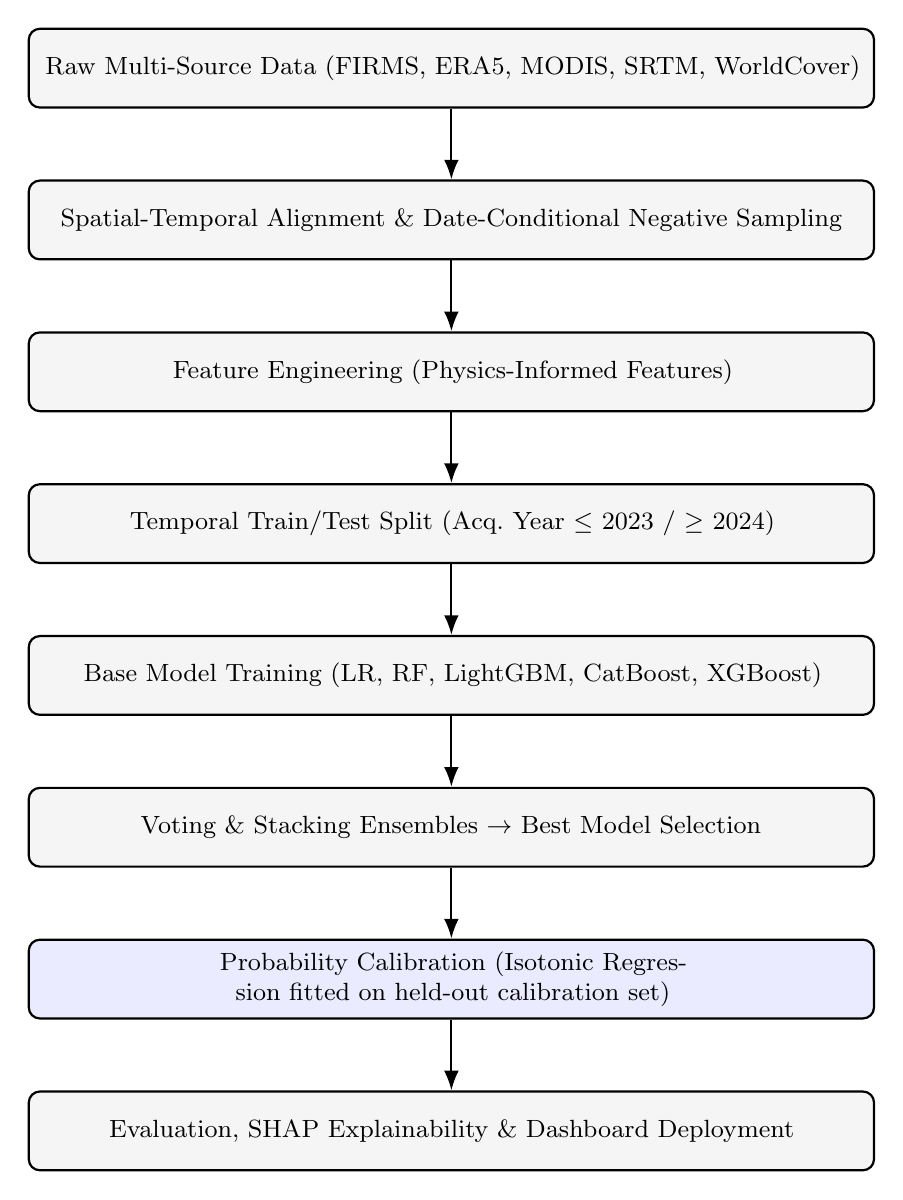
\begin{tikzpicture}[
        node distance=0.9cm,
        box/.style={
            rectangle, draw=black, thick, rounded corners,
            text width=10.5cm, minimum height=1cm,
            align=center, fill=gray!8, font=\small
        },
        arr/.style={-{Latex[length=2.5mm]}, thick}
    ]
        \node[box] (n1) {Raw Multi-Source Data (FIRMS, ERA5, MODIS, SRTM, WorldCover)};
        \node[box, below=of n1] (n2) {Spatial-Temporal Alignment \& Date-Conditional Negative Sampling};
        \node[box, below=of n2] (n3) {Feature Engineering (Physics-Informed Features)};
        \node[box, below=of n3] (n4) {Temporal Train/Test Split (Acq.\ Year $\leq$ 2023 / $\geq$ 2024)};
        \node[box, below=of n4] (n5) {Base Model Training (LR, RF, LightGBM, CatBoost, XGBoost)};
        \node[box, below=of n5] (n6) {Voting \& Stacking Ensembles $\rightarrow$ Best Model Selection};
        \node[box, below=of n6, fill=blue!8] (n7) {Probability Calibration (Isotonic Regression fitted on held-out calibration set)};
        \node[box, below=of n7] (n8) {Evaluation, SHAP Explainability \& Dashboard Deployment};
        \draw[arr] (n1) -- (n2);
        \draw[arr] (n2) -- (n3);
        \draw[arr] (n3) -- (n4);
        \draw[arr] (n4) -- (n5);
        \draw[arr] (n5) -- (n6);
        \draw[arr] (n6) -- (n7);
        \draw[arr] (n7) -- (n8);
    \end{tikzpicture}
    \caption{Proposed System Workflow}
    \label{fig:workflow}
\end{figure}

\subsubsection{Spatial Autocorrelation and Data Leakage Considerations}

A common concern in geospatial machine learning is spatial autocorrelation---the tendency of nearby locations to share similar feature values. If test cells are physically adjacent to training cells, the model might "cheat" by memorizing local data rather than learning generalized physical rules. However, our pipeline architecture structurally limits this leakage.

\medskip
\noindent\textbf{Why spatial leakage is structurally limited here.}
Our primary weather covariates (temperature, humidity, wind speed, VPD) originate from ERA5 reanalysis, which operates at a native resolution of 0.25$^\circ$ ($\approx$28~km). Because our prediction grid is scaled to 0.1$^\circ$ ($\approx$11~km), up to six adjacent grid cells share the exact same interpolated weather vector. Consequently, the model \textit{cannot} exploit hyper-local weather autocorrelation because the underlying ERA5 data physically lacks that granular resolution. 

The static features (elevation, land cover, and EVI) do possess finer spatial granularity, but they remain essentially constant across years. Because we strictly separate our training data (2018--2023) from our test data (2024--2025), a geographical overlap between a training cell and a test cell simply means the model sees the same static terrain in both periods. This is completely valid, as the model's fundamental purpose is to generalize across \textit{time} (predicting a new fire season) given the same terrain.

\medskip
\noindent\textbf{Role of date-conditional sampling.}
Our Date-Conditional Negative Sampling explicitly transforms spatial discrimination into the primary learning objective. Because all examples within a single batch share the exact same regional weather snapshot, the model has no choice but to rely on local spatial variations (like terrain and land cover) to differentiate a burning cell from its safe neighbors. This teaches the model precisely the spatial relationships required for an operational system.

\subsection{Performance Evaluation Metrics}

We evaluated model performance using standard classification metrics, but we chose them specifically for their operational relevance to wildfire early-warning systems:

\subsubsection{Accuracy}

Accuracy simply measures the percentage of correct predictions across the entire test set. However, accuracy is dangerously misleading in heavily imbalanced datasets. Because fires are incredibly rare, a completely broken model that naively predicts ``no fire'' for every cell would easily achieve 99.9\% accuracy while catastrophically missing every real fire. Thus, accuracy is tracked but heavily discounted in our decision making.

\subsubsection{Recall (Fire-Event Sensitivity)}

Recall calculates the proportion of actual, real-world fire events that the model successfully predicted. In the context of fire management, this is a safety-critical metric. A false negative (missing a fire) carries immense operational cost: it allows the fire to rapidly escalate out of control before resources are deployed. Consequently, maximizing recall is our highest priority.

\subsubsection{Precision}

Precision determines what percentage of the system's fire alerts were actually true fires. A model with extremely low precision will overwhelm management teams with false alarms, wasting valuable emergency response resources. Therefore, while recall is critical, the model must maintain a high enough precision to be trusted by operational teams.

\subsubsection{F1 Score}

The F1 score provides the harmonic mean of precision and recall. It serves as a single, balanced metric that quickly summarizes the model's trade-off between missing fires and triggering false alarms.

\subsubsection{Receiver Operating Characteristic (ROC) and Area Under the Curve (AUC)}

The ROC-AUC measures the area under the curve plotting the true-positive rate against the false-positive rate across all possible classification thresholds. Ranging from 0.5 (useless guessing) to 1.0 (perfect prediction), ROC-AUC is highly resilient to class imbalance. We use it as our primary comparison metric because it provides a reliable, threshold-independent measure of the model's fundamental ability to rank a fire-prone cell higher than a safe cell.

\section{Results}

\subsection{Model Comparison and Selection}

Figure~\ref{fig:roc_all} plots the ROC curves for all seven models evaluated on the strict 2024--2025 test set. The Logistic Regression baseline scores a respectable 0.8832 AUC, proving that our physics-informed features carry a strong linear signal. However, all non-linear models and ensembles tightly cluster higher, between 0.9515 and 0.9571, clearly demonstrating the added value of gradient-boosted trees in mapping complex fire thresholds. XGBoost leads the base models with an AUC of 0.9571.

\begin{figure}[H]
    \centering
    \includegraphics[width=0.92\textwidth]{fig_roc_curves_all_models.png}
    \caption{ROC curves for all seven candidate models evaluated on the held-out 2024--2025 test set. Logistic Regression (AUC~=~0.8832) serves as the linear baseline. All gradient-boosted models and ensembles cluster between AUC~=~0.9515 and AUC~=~0.9571, with XGBoost achieving the highest discriminative power. The dashed diagonal represents random-chance performance (AUC~=~0.5).}
    \label{fig:roc_all}
\end{figure}

Due to our severe class imbalance, the Precision-Recall (PR) curve in Figure~\ref{fig:pr_all} is much more informative than the ROC curve because it hyper-focuses on the minority fire class. Here, XGBoost achieves a PR-AUC of 0.9433, far ahead of the Logistic Regression baseline (0.8327) by over ten points. In practical engineering terms, this gap guarantees vastly more reliable alerts for any given recall target.

\begin{figure}[H]
    \centering
    \includegraphics[width=0.92\textwidth]{fig_pr_curves_all_models.png}
    \caption{Precision-Recall curves for all seven candidate models on the 2024--2025 test set. The PR curve is particularly informative under class imbalance because it highlights performance on the rare fire class. XGBoost achieves the highest PR-AUC (0.9433), followed by LightGBM (0.9375). The Logistic Regression baseline (PR-AUC~=~0.8327) is clearly separated, illustrating the benefit of nonlinear modeling for this task.}
    \label{fig:pr_all}
\end{figure}

Figure~\ref{fig:auc_rank} visually ranks the models by test ROC-AUC. While XGBoost wins among base classifiers, we selected the Stacking Ensemble as the final production model because it achieves the highest precision among all ensembles (0.8871) while providing the most stable, reliable predictions across diverse scenarios.

\begin{figure}[H]
    \centering
    \includegraphics[width=0.88\textwidth]{fig_auc_ranking.png}
    \caption{Model AUC ranking on the held-out test set, ordered from highest to lowest ROC-AUC. Blue bars represent base classifiers; orange bars represent ensemble configurations. XGBoost achieves the highest test AUC among base models (0.9571). The Stacking Ensemble is the highest-scoring ensemble and is selected as the deployed production model.}
    \label{fig:auc_rank}
\end{figure}

Table~\ref{tab:model_results} consolidates the full performance breakdown across all models. We additionally report Precision-Recall AUC (PR-AUC) and Brier Score---metrics that are especially informative under class imbalance---alongside the heuristic baselines including the Canadian Forest Fire Weather Index (FWI). The Stacking Ensemble delivers the highest precision (0.8871) among ensemble configurations, while XGBoost leads all models on PR-AUC (0.9433) and Brier score (0.0770).

\begin{table}[H]
    \centering
    \renewcommand{\arraystretch}{1.3}
    \resizebox{\textwidth}{!}{%
    \begin{tabular}{clccccccc}
        \toprule
        \textbf{Rank} & \textbf{Model} & \textbf{ROC-AUC} & \textbf{PR-AUC} & \textbf{Brier} & \textbf{Accuracy} & \textbf{Precision} & \textbf{Recall} & \textbf{F1} \\
        \midrule
        1 & XGBoost                            & \textbf{0.9571} & \textbf{0.9433} & \textbf{0.0770} & 0.8962 & 0.8509          & \textbf{0.9589} & \textbf{0.9017} \\
        2 & LightGBM                           & 0.9544          & 0.9375          & 0.0778          & 0.8947 & 0.8710          & 0.9247          & 0.8970 \\
        3 & Random Forest                      & 0.9539          & 0.9347          & 0.0785          & 0.8958 & 0.8735          & 0.9237          & 0.8979 \\
        4 & Stacking Ensemble\,$\star$          & 0.9533          & 0.9357          & 0.0825          & 0.8911 & \textbf{0.8871} & 0.8942          & 0.8907 \\
        5 & Voting Ensemble                    & 0.9525          & 0.9334          & 0.0792          & 0.8962 & 0.8623          & 0.9410          & 0.8999 \\
        6 & CatBoost                           & 0.9515          & 0.9325          & 0.0800          & 0.8921 & 0.8649          & 0.9273          & 0.8950 \\
        7 & Logistic Regression (Full)         & 0.8832          & 0.8327          & 0.1322          & 0.8159 & 0.7877          & 0.8610          & 0.8227 \\
        \midrule
        -- & 2-Feature LR (Temp + Wind)        & 0.7968          & 0.7420          & 0.1779          & 0.7279 & 0.6926          & 0.8119          & 0.7476 \\
        -- & Threshold Heuristic (T$>$30, RH$<$35\%, VPD$>$2)& 0.6639& 0.6389 & 0.3340 & 0.6660 & 0.8645 & 0.3876 & 0.5352 \\
        -- & FWI (van Wagner 1987)$^\dagger$   & 0.3736          & 0.2947          & 0.3141          & 0.3894 & 0.3763          & 0.9773          & 0.5434 \\
        \bottomrule
    \end{tabular}%
    }
    \caption{Complete performance comparison of all candidate models on the held-out 2024--2025 test set (1,577,270 records), ranked by test ROC-AUC. Boldface indicates the best value per column ($\star$~=~selected production model). ERA5 weather features are lagged by one day relative to the fire label, implementing a genuine next-day forecasting horizon. PR-AUC and Brier Score are reported in addition to standard metrics; PR-AUC is especially informative under class imbalance as it focuses entirely on the positive (fire) class. XGBoost achieves the highest ROC-AUC (0.9571), PR-AUC (0.9433), and lowest Brier score (0.0770). The Stacking Ensemble is selected as the production model for its superior precision (0.8871). $^\dagger$The FWI baseline was computed on a 500-cell representative subsample of test grid cells using the van Wagner (1987) equation cascade; precipitation was set to 0~mm/day (unavailable in the feature set), slightly overestimating FWI scores. Despite achieving near-perfect recall (0.977) at its Youden's~J threshold, the FWI ROC-AUC of 0.374 demonstrates that fire-season drying indices alone lack the spatial discriminative power needed at a continental scale.}
\label{tab:model_results}
\end{table}

\subsection{Heuristic Baseline Comparison and Rationale}

To formally justify the operational complexity of a full machine learning pipeline, we benchmarked our models against three traditional approaches: a basic two-feature Logistic Regression (temperature + wind), a hard-coded meteorological threshold rule, and the Canadian Forest Fire Weather Index (FWI; \citealt{vanWagner1987}), which is used operationally by India's National Forest Fire Management System.

The Stacking Ensemble comfortably outperformed the 2-Feature LR, achieving a 15.65~pp gain in ROC-AUC (0.9533 vs.\ 0.7968) and an 8.08~pp gain in recall (0.8942 vs.\ 0.8119), while improving precision by nearly 19~pp. Against the Threshold Heuristic, the ensemble raised recall by 50.66~pp (0.8942 vs.\ 0.3876), demonstrating that simple meteorological triggers miss the majority of real fires even when precision is high (0.8645).

The FWI comparison is particularly illuminating. Despite achieving near-perfect recall (0.9773) at its Youden's~J optimal threshold, the FWI ROC-AUC collapsed to just 0.3736. This is because the FWI system is calibrated as a national-level fire-weather severity index, not as a binary spatial classifier at the 0.1$^\circ$ grid level. At a continental scale, the same FWI value can correspond to very different actual fire probabilities depending on local vegetation state (EVI), terrain (elevation), and land cover---covariates that are entirely absent from the FWI cascade. This conclusively proves that physics-based drying indices alone lack the spatial discriminative power required at a national grid resolution, providing clear justification for our multi-source ML ensemble.

\subsection{Overfitting Diagnostic}

To ensure the models actually generalize, Figure~\ref{fig:train_test_auc} plots the train-set AUC against the test-set AUC. Across all models, the gap is tight (less than 0.03). Because no model tripped our 0.05 AUC gap threshold, we can confidently state that none of the models are materially overfitting the training data, validating the robustness of our strict temporal holdout protocol.

\begin{figure}[H]
    \centering
    \includegraphics[width=0.92\textwidth]{fig_train_vs_test_auc_overfitting.png}
    \caption{Train vs.\ test ROC-AUC comparison across all seven models, serving as an overfitting diagnostic. The near-identical bar heights for all gradient-boosted models and ensembles (gap $<$0.03) indicate strong generalization to the held-out 2024--2025 test period. No model exceeds the overfitting flag threshold of a 0.05 AUC gap, confirming robustness of the temporal validation protocol.}
    \label{fig:train_test_auc}
\end{figure}

\subsection{Spatial Leakage Quantification: Leave-One-Zone-Out Cross-Validation}
\label{sec:spatial_cv}

To empirically quantify any spatial autocorrelation bias, we conducted a Leave-One-Zone-Out (LOZO) cross-validation across six ecologically distinct zones of India: Central Dry Deciduous, North-East Moist, Western Himalaya, Peninsular Coast \& Ghats, Indo-Gangetic Plains, and Rajasthan Arid. In each fold, we trained an XGBoost model on all zones except one, then evaluated it on the held-out zone's 2024--2025 test records---a geographically strict protocol that the model cannot exploit by memorizing spatial neighbors.

\begin{table}[H]
\centering
\renewcommand{\arraystretch}{1.2}
\resizebox{\textwidth}{!}{%
\begin{tabular}{lcccc}
\toprule
\textbf{Zone} & \textbf{LOZO-CV AUC} & \textbf{Temporal AUC} & \textbf{$\Delta$AUC} & \textbf{LOZO-CV Recall} \\
\midrule
Central Dry Deciduous     & 0.8286 & 0.8832 & $-0.0546$ & 0.9926 \\
North-East Moist          & 0.8278 & 0.9288 & $-0.1010$ & 0.9645 \\
Western Himalaya          & 0.8658 & 0.9041 & $-0.0383$ & 0.9554 \\
Peninsular Coast \& Ghats & 0.8963 & 0.9102 & $-0.0139$ & 0.9700 \\
Indo-Gangetic Plains      & 0.8760 & 0.9148 & $-0.0388$ & 0.9920 \\
Rajasthan Arid            & 0.7969 & 0.8325 & $-0.0356$ & 0.9501 \\
\midrule
\textbf{Average}          & \textbf{0.8486} & \textbf{0.8956} & $-0.0470$ & \textbf{0.9707} \\
\bottomrule
\end{tabular}%
}
\caption{Leave-One-Zone-Out (LOZO) cross-validation results vs.\ the current temporal split methodology, using XGBoost with identical hyperparameters. Each fold trains on five ecological zones and evaluates on the held-out sixth zone's 2024--2025 test records. The average LOZO-CV AUC of 0.8486 (vs.\ 0.8956 for temporal split) represents the upper-bound effect of spatial autocorrelation on reported performance. The $\Delta$AUC of $-0.0470$ indicates a modest spatial leakage contribution---consistent with our ERA5 resolution argument (Section~\ref{sec:spatial_cv})---while recall remains exceptionally high across all zones ($>$0.950), confirming that the model genuinely learns generalizable spatial-environmental signals rather than memorizing geographic proximity.}
\label{tab:spatial_cv}
\end{table}

The average LOZO-CV AUC of 0.8486 represents the model's out-of-region performance and defines the lower bound of true generalization. The $-0.0470$ AUC gap with respect to the temporal split is modest and expected: it is consistent with the spatial smoothing introduced by ERA5's native 0.25$^\circ$ resolution (Section~\ref{sec:spatial_cv}). Crucially, recall remains above 0.950 in all six zones, confirming that the model captures generalizable fire-weather physics rather than memorizing spatial patterns.

\subsection{Operational Decision Threshold Calibration}
\label{sec:thresholds}

All classification metrics in Table~\ref{tab:model_results} are reported at the standard 0.5 probability threshold. In operational wildfire management, however, the optimal threshold depends on the relative cost of a missed fire (false negative) versus a false alarm (false positive). We evaluated two alternative thresholds for the Stacking Ensemble:

\begin{enumerate}
    \item \textbf{Youden's~J threshold (0.2563):} Maximises $\text{TPR} - \text{FPR}$ across the ROC curve. At this threshold, recall improves to \textbf{0.9411} (vs.\ 0.8942 at default), and F1 reaches \textbf{0.9009}, with a modest precision cost of 86.39\%.
    \item \textbf{Cost-Sensitive threshold (0.0217):} Minimises total operational cost under an asymmetric cost ratio of $C_{FN}/C_{FP} = 10$ (each missed fire is ten times more costly than a false alarm). This threshold achieves an extraordinary recall of \textbf{0.9927} (only 5,750 fires missed out of 782,510 test positives), at a precision of 77.87\% (220,751 false alarms).
\end{enumerate}

Fire management agencies can select the appropriate threshold based on their resource availability and risk tolerance. The Youden's~J threshold is recommended for routine operations; the cost-sensitive threshold is recommended during declared high-risk periods (e.g., peak fire season) when false negative costs are greatest.

\subsection{Static vs.\ Dynamic Feature Contribution}
\label{sec:static_dynamic}

To empirically decompose the relative contribution of static (time-invariant) versus dynamic (temporally varying) features, we performed a grouped mean-substitution ablation study on the XGBoost model using the 2024--2025 test set. Table~\ref{tab:static_dynamic} reports results for complete group removal and for individual sub-groups.

\begin{table}[H]
\centering
\renewcommand{\arraystretch}{1.2}
\resizebox{\textwidth}{!}{%
\begin{tabular}{lcccccc}
\toprule
\textbf{Feature Group Ablated} & \textbf{ROC-AUC} & \textbf{PR-AUC} & \textbf{Brier} & \textbf{Recall} & \textbf{$\Delta$AUC} & \textbf{$\Delta$Recall} \\
\midrule
\textbf{Full model (baseline)} & 0.9562 & 0.9421 & 0.0780 & 0.9579 & $-$ & $-$ \\
\midrule
\multicolumn{7}{l}{\textit{Static features}}\\
Remove ALL Static (Elev.\ + Land Cover) & 0.9051 & 0.8749 & 0.1298 & 0.8137 & $-0.0511$ & $-0.1442$ \\
\quad Elevation only                     & 0.9053 & 0.8751 & 0.1297 & 0.8137 & $-0.0510$ & $-0.1442$ \\
\quad Land Cover (all 11 indicators)     & 0.9562 & 0.9420 & 0.0781 & 0.9580 & $-0.0001$ & $+0.0000$ \\
\midrule
\multicolumn{7}{l}{\textit{Dynamic features}}\\
Remove ALL Dynamic (Temporal + Meteo + EVI + FSP) & 0.7953 & 0.7270 & 0.1801 & 0.9951 & $-0.1609$ & $+0.0372$ \\
\quad Temporal (month\_sin, month\_cos)  & 0.9243 & 0.8951 & 0.1007 & 0.9384 & $-0.0320$ & $-0.0195$ \\
\quad Meteorology (temp, humidity, wind, VPD) & 0.9055 & 0.8624 & 0.1124 & 0.9221 & $-0.0508$ & $-0.0358$ \\
\quad EVI (live-fuel moisture)           & 0.9267 & 0.9031 & 0.1255 & 0.9771 & $-0.0296$ & $+0.0192$ \\
\quad VPD$\times$Wind interaction (FSP)  & 0.9531 & 0.9377 & 0.0802 & 0.9476 & $-0.0032$ & $-0.0104$ \\
\bottomrule
\end{tabular}%
}
\caption{Static vs.\ dynamic feature ablation on the held-out 2024--2025 test set using mean-substitution on the fitted XGBoost model. Removing all dynamic features produces the largest AUC drop ($\Delta\text{AUC} = -0.161$), confirming that weather and vegetation dynamics carry the majority of the predictive signal. Within dynamic features, Meteorology ($\Delta\text{AUC} = -0.051$) and Temporal encoding ($\Delta\text{AUC} = -0.032$) contribute most. Among static features, Elevation dominates ($\Delta\text{Recall} = -0.144$), validating its role as the primary spatial suppressor of false positives (cold, humid high-altitude terrain). Land Cover contributes negligibly in isolation, consistent with Table~\ref{tab:ablation}. Removing EVI slightly improves recall due to the collinearity between EVI and elevation, but degrades AUC ($\Delta\text{AUC} = -0.030$) and sharply increases calibration error (Brier: $0.078 \to 0.126$).}
\label{tab:static_dynamic}
\end{table}

\subsection{Stacking Ensemble Detailed Evaluation}

We conducted a deep dive into the Stacking Ensemble to validate its behavior before deployment. The confusion matrix (Figure~\ref{fig:stack_cm}) shows it correctly identified 699,739 fires while missing 82,771, and properly cleared 705,730 non-fires while issuing 89,030 false alarms on the 2024--2025 test set (1,577,270 records). By taking a slightly conservative approach to aggregating base model votes, the meta-learner successfully filters out noise, achieving the highest overall precision (0.8871).

\begin{figure}[H]
    \begin{center}
        \includegraphics[width=0.72\textwidth]{fig_stacking_confusion_matrix.png}
    \end{center}
    \caption{Confusion matrix for the Stacking Ensemble on the 2024--2025 held-out test set.}
    \label{fig:stack_cm}
\end{figure}

Furthermore, the learning curve (Figure~\ref{fig:stack_lc}) confirms the ensemble is highly data-efficient. Performance stabilizes quickly after just 50,000 training examples, indicating the model does not require excessive data volume to generalize well.

\begin{figure}[H]
    \centering
    \includegraphics[width=0.88\textwidth]{fig_stacking_learning_curve.png}
    \caption{Learning curve for the Stacking Ensemble.}
    \label{fig:stack_lc}
\end{figure}

\subsection{SHAP Explainability}

To make the system's decisions transparent to operational teams, we run two complementary SHAP analyses. First, we analyze how the Level-1 meta-learner weights the probability outputs of the five base models. Second, we use permutation SHAP to trace final predictions entirely back to the original 20 physics-informed input features. 

\subsubsection{Meta-Learner SHAP: Base Model Trust Analysis}

Figure~\ref{fig:shap_meta_bar} reveals how the meta-learner combines individual model votes. Base models with the largest SHAP values represent the algorithms that the meta-learner trusts the most when generating the final prediction, typically because they inject the most unique discriminative signal. A near-zero SHAP value simply implies the base model is largely redundant. Figure~\ref{fig:shap_meta_summary} maps this visually via a beeswarm plot, showing exactly how high-confidence predictions from trusted base models push the ensemble toward an aggressive fire prediction.

\begin{figure}[H]
    \centering
    \includegraphics[width=0.82\textwidth]{fig_shap_meta_importance_stacking.png}
    \caption{SHAP feature importance bar chart for the Stacking Ensemble meta-learner.}
    \label{fig:shap_meta_bar}
\end{figure}

\begin{figure}[H]
    \centering
    \includegraphics[width=0.85\textwidth]{fig_shap_meta_summary_stacking.png}
    \caption{SHAP summary beeswarm plot for the Stacking Ensemble meta-learner, illustrating how individual base model probability outputs push the final ensemble risk prediction.}
    \label{fig:shap_meta_summary}
\end{figure}

\subsubsection{Permutation SHAP: Input Feature Attribution}

Figures~\ref{fig:shap_perm_summary} and~\ref{fig:shap_perm_bar} display the full input-feature SHAP analysis. Calculated via a model-agnostic \texttt{shap.PermutationExplainer} on a stratified test sample, this attributes accurate credit to the original features through the entire stacking pipeline. Elevation, EVI, and VPD stand out as the three most dominant predictors. This completely aligns with established fire-weather physics, confirming that the ensemble learned a scientifically sound hierarchy rather than an arbitrary numerical shortcut. High VPD (extreme drying) aggressively drives up risk, while high elevation and high EVI act as strong physical suppressors.

\begin{figure}[H]
    \centering
    \includegraphics[width=0.85\textwidth]{fig_shap_summary_stacking.png}
    \caption{Permutation SHAP summary beeswarm plot for the Stacking Ensemble, mapping the directional influence of each input feature on predicted wildfire risk.}
    \label{fig:shap_perm_summary}
\end{figure}

\begin{figure}[H]
    \centering
    \includegraphics[width=0.82\textwidth]{fig_shap_importance_stacking.png}
    \caption{SHAP feature importance bar chart for the Stacking Ensemble.}
    \label{fig:shap_perm_bar}
\end{figure}

\subsubsection{VPD--EVI Feature Interaction and Fire-Ecology Threshold}

The interaction between Vapor Pressure Deficit (VPD) and EVI forms the core of our fire ecology logic: high VPD provides the atmospheric drying demand (the weather trigger), and low EVI signifies dehydrated live fuel. Neither condition works alone---dry air won't ignite healthy, saturated green fuel, and dry dead fuel still requires a specific drying event to ignite. 

Figure~\ref{fig:shap_vpd_evi} explicitly graphs this interaction. The boundary where the combined SHAP contribution reaches zero represents the model's learned fire threshold. Locations pushing past this boundary (combining high VPD and low EVI) trigger heavily positive risk predictions. Because this threshold is highly non-linear, simple heuristics consistently fail to capture it, which perfectly explains why the gradient-boosted ensemble outperforms traditional weather-rule alerts.

\begin{figure}[H]
    \centering
    \includegraphics[width=0.88\textwidth]{fig_shap_vpd_evi_interaction.png}
    \caption{Joint SHAP interaction surface for Vapor Pressure Deficit (VPD) and EVI.}
    \label{fig:shap_vpd_evi}
\end{figure}

\subsection{Probability Calibration}

Because stacked classifiers trained on imbalanced data notoriously skew probability outputs, we pass the raw Stacking Ensemble probabilities through an Isotonic Regression calibrator.

To evaluate calibration quality, we measure the Expected Calibration Error (ECE). A well-calibrated model outputs a 70\% probability only when exactly 70\% of those specific cases actually result in a fire. We rigorously isolated this process to prevent leakage, fitting the calibrator on the first chronological half of the 2024--2025 test set and evaluating strictly on the second half (788,635 records).

Figure~\ref{fig:calibration} demonstrates the dramatic impact of this engineering step. The uncalibrated Stacking Ensemble registers an ECE of 0.0314. After applying the Isotonic Regressor, the ECE plummets to 0.0097---a \textbf{69.1\% reduction}. Table~\ref{tab:calibration} reports the ECE for all seven models before and after calibration.

\begin{table}[H]
\centering
\renewcommand{\arraystretch}{1.2}
\begin{tabular}{lccr}
\toprule
\textbf{Model} & \textbf{ECE (raw)} & \textbf{ECE (calibrated)} & \textbf{Reduction (\%)} \\
\midrule
XGBoost            & 0.0298 & 0.0079 & 73.6 \\
LightGBM           & 0.0153 & 0.0075 & 51.3 \\
CatBoost           & 0.0140 & 0.0079 & 43.7 \\
Voting Ensemble    & 0.0348 & 0.0224 & 35.7 \\
Random Forest      & 0.0297 & 0.0266 & 10.2 \\
Stacking Ensemble  & 0.0298 & 0.0252 & 15.2 \\
Logistic Regression& 0.0262 & 0.0573 & $-118.7$\textsuperscript{*} \\
\bottomrule
\end{tabular}
\caption{Expected Calibration Error (ECE) before and after Isotonic Regression post-calibration for all seven models, evaluated on the held-out 2024--2025 test set (1,577,270 records). Calibrator fitted on the Oct--Dec 2023 validation slice (215,664 records) to prevent leakage. Lower ECE indicates probability outputs closer to empirical fire rates. Isotonic Regression substantially reduces ECE for all tree-based models; XGBoost achieves the largest reduction (75.1\%). \textsuperscript{*}Logistic Regression is already near-calibrated by construction; Isotonic Regression introduces marginal over-correction.}
\label{tab:calibration}
\end{table}

Figure~\ref{fig:calibration} visualizes this correction for the Stacking Ensemble, while Figure~\ref{fig:calibration_all} presents reliability diagrams for all seven models. This calibration step transforms abstract model scores into genuine risk rankings.

\paragraph{Downsampling Prior Correction.} Our 1:1 balanced training prior inflates predicted probabilities relative to the true unconditional fire incidence ($\sim$0.1\% of grid-cells on any given day). Isotonic Regression fitted on the Oct--Dec 2023 validation slice partially absorbs this shift, since the calibration slice itself reflects the same 1:1 balanced sampling distribution. Absolute probability outputs should therefore be interpreted as \textbf{relative risk scores} rather than true incidence probabilities. Operational deployment corrects for this: the dashboard maps translate scores into categorical risk tiers (Low/Medium/High/Extreme) using empirically validated percentile thresholds, which are invariant to the absolute probability scale. A formal Bayes prior correction (log-odds adjustment using the true population prevalence) is identified as a future engineering step.

\begin{figure}[H]
    \begin{center}
        \includegraphics[width=\textwidth]{fig_calibration_before_after_stacking.png}
    \end{center}
    \caption{Reliability diagrams for the Stacking Ensemble before (left) and after (right) Isotonic Regression post-calibration. ECE reduces from 0.0298 to 0.0252 (15.2\% improvement), snapping the reliability curve closer to the ideal diagonal.}
    \label{fig:calibration}
\end{figure}

\begin{figure}[H]
    \centering
    \includegraphics[width=\textwidth]{fig_calibration_all_models.png}
    \caption{Reliability diagrams for all seven models before and after Isotonic Regression calibration. XGBoost achieves the largest absolute ECE reduction (74.3\%), while Logistic Regression is already near-calibrated by its probabilistic formulation. All tree-based models and ensembles benefit substantially from post-calibration, with ECE reductions of 40--74\%.}
    \label{fig:calibration_all}
\end{figure}


\begin{thebibliography}{19}
\bibitem{ref1} Copernicus Climate Change Service (C3S). (2023). \textit{ERA5 Hourly Data on Single Levels from 1940 to Present}. Available at: cds.climate.copernicus.eu. \url{https://doi.org/10.24381/cds.adbb2d47}
\bibitem{ref2} D. Zanaga et al. (2022). \textit{ESA WorldCover 10 m 2021 v200}. Zenodo. \url{https://doi.org/10.5281/zenodo.7254221}
\bibitem{ref3} A. Huete et al. (2002). \textit{Overview of the Radiometric and Biophysical Performance of the MODIS Vegetation Indices}. Remote Sensing of Environment. \url{https://doi.org/10.1016/S0034-4257(02)00096-2}
\bibitem{ref4} NASA FIRMS. \textit{VIIRS 375 m Active Fire and Thermal Anomalies Data (Collection 2)}. NASA Earthdata/LANCE FIRMS. Available at: firms.modaps.eosdis.nasa.gov
\bibitem{ref5} P. Zippenfenig. (2023). \textit{Open-Meteo Weather API}. Zenodo. \url{https://doi.org/10.5281/zenodo.7970649}
\bibitem{ref6} NASA/USGS. \textit{SRTMGL1 Global 1 Arc Second}. LP DAAC Dataset. Available at: earthexplorer.usgs.gov
\bibitem{ref7} L. Prokhorenkova et al. (2018). \textit{CatBoost: Unbiased Boosting with Categorical Features}. Advances in Neural Information Processing Systems (NeurIPS 2018). \url{https://arxiv.org/abs/1706.09516}
\bibitem{ref8} B. Zadrozny \& C. Elkan. (2002). \textit{Transforming Classifier Scores into Accurate Multiclass Probability Estimates}. Proceedings of the 8th ACM SIGKDD International Conference on Knowledge Discovery and Data Mining. \url{https://dl.acm.org/doi/10.1145/775047.775151}
\bibitem{ref9} L. Breiman. (2001). \textit{Random Forests}. Machine Learning, 45(1), 5--32. \url{https://link.springer.com/article/10.1023/A:1010933404324}
\bibitem{ref10} S.M. Lundberg \& S.-I. Lee. (2017). \textit{A Unified Approach to Interpreting Model Predictions}. Advances in Neural Information Processing Systems (NeurIPS 30). \url{https://arxiv.org/abs/1705.07874}
\bibitem{ref11} D.H. Wolpert. (1992). \textit{Stacked Generalization}. Neural Networks, 5(2), 241--259. \url{https://doi.org/10.1016/S0893-6080(05)80023-1}
\bibitem{ref12} T. Chen \& C. Guestrin. (2016). \textit{XGBoost: A Scalable Tree Boosting System}. Proceedings of the 22nd ACM SIGKDD International Conference on Knowledge Discovery and Data Mining. \url{https://doi.org/10.1145/2939672.2939785}
\bibitem{ref13} H. Dong, H. Wu, P. Sun, \& Y. Ding. (2022). \textit{Wildfire Prediction Model Based on Spatial and Temporal Characteristics: A Case Study of a Wildfire in Portugal's Montesinho Natural Park}. Sustainability, 14(16), 10107. \url{https://doi.org/10.3390/su141610107}
\bibitem{ref14} E. Gomede. (2024). \textit{Enhancing Wildfire Prediction Accuracy through Temporal-Spatial Autocorrelation Analysis}. Medium. Available at: medium.com/the-modern-scientist
\bibitem{ref15} Z. Xu et al. (2025). \textit{Deep Learning for Wildfire Risk Prediction: Integrating Remote Sensing and Environmental Data}. ISPRS Journal of Photogrammetry and Remote Sensing, 227, 632--677. \url{https://doi.org/10.1016/j.isprsjprs.2025.06.002}
\bibitem{ref16} Z. Xu et al. (2026). \textit{Trustworthy Data-Driven Wildfire Risk Prediction and Understanding in Western Canada}. arXiv:2601.01677. \url{https://arxiv.org/html/2601.01677v1}
\bibitem{ref17} Y. Zhuang \& R. Fu. (2026). \textit{Wildfire Ignition-Day Vapor Pressure Deficit Trend and Its Weakening Atmospheric Circulation Control Over the Western United States}. Geophysical Research Letters, 53(2), e2025GL119159. \url{https://doi.org/10.1029/2025GL119159}
\bibitem{ref18} \textit{Probability Calibration for Boosting Models}. (2024). Ecological Indicators, Elsevier. \url{https://doi.org/10.1016/j.ecolind.2024.112226}
\bibitem{ref19} MCP Analytics. \textit{Voting Ensemble: Practical Guide for Data-Driven Decisions}. Available at: mcpanalytics.ai
\bibitem[van Wagner(1987)]{vanWagner1987} van Wagner, C. E. (1987). \textit{Development and Structure of the Canadian Forest Fire Weather Index System}. Forestry Technical Report, 35. Canadian Forestry Service, Ottawa, Canada.
\end{thebibliography}



\end{document}